%%%% Paramétrage du TD %%%%

\def\xxnumchapitre{Chapitre 2 \vspace{.2cm}}
\def\xxchapitre{\hspace{.12cm} Révisions SLCI}

\def\xxcompetences{%
\textsl{%
\textbf{Savoirs et compétences :}\\
\vspace{-.4cm}
\begin{itemize}[label=\ding{112},font=\color{bleuxp}] 
\item .
%\item \textit{Mod3.C2 : } pôles dominants et réduction de l’ordre du modèle : principe, justification
\end{itemize}
}}


\def\xxfigures{
%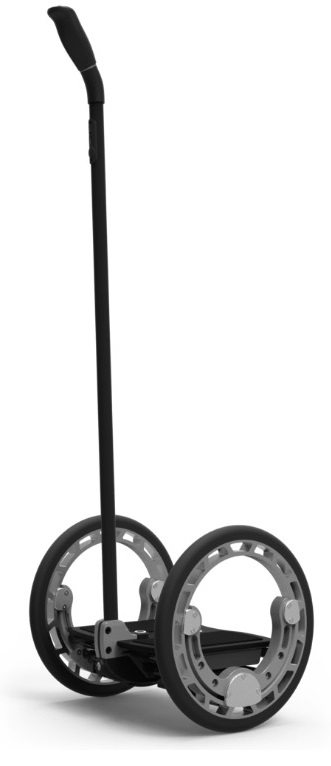
\includegraphics[width=3cm]{fig_01}\\
%\textit{}
}%figues de la page de garde

\def\xxtitreexo{Banc d'essai BTP}
\def\xxsourceexo{\hspace{.2cm} \footnotesize{Concours CCINP-- TSI 20??}}
\def\xxactivite{{TD 01} \ifprof  -- Corrigé \else \fi}

%\iflivret
\input{../../../Style/pagegarde_TD}
%\else
%\pagestyle{empty}


%%%%%%%% PAGE DE GARDE COURS
\ifcours
\begin{tikzpicture}[remember picture,overlay]
\node at (current page.north west)
{\begin{tikzpicture}[remember picture,overlay]
\node[anchor=north west,inner sep=0pt] at (0,0) {\includegraphics[width=\paperwidth]{\thechapterimage}};
\draw[anchor=west] (-2cm,-8cm) node [line width=2pt,rounded corners=15pt,draw=ocre,fill=white,fill opacity=0.6,inner sep=40pt]{\strut\makebox[22cm]{}};
\draw[anchor=west] (1cm,-8cm) node {\huge\sffamily\bfseries\color{black} %
\begin{minipage}{1cm}
\rotatebox{90}{\LARGE\sffamily\textsc{\color{ocre}\textbf{\xxnumpartie}}}
\end{minipage} \hfill
\begin{minipage}[c]{14cm}
\begin{titrepartie}
\begin{flushright}
\renewcommand{\baselinestretch}{1.1} 
\Large\sffamily\textsc{\textbf{\xxpartie}}
\renewcommand{\baselinestretch}{1} 
\end{flushright}
\end{titrepartie}
\end{minipage} \hfill
\begin{minipage}[c]{3.5cm}
{\large\sffamily\textsc{\textbf{\color{ocre} \discipline}}}
\end{minipage} 
 };
\end{tikzpicture}};
\end{tikzpicture}


\begin{tikzpicture}[overlay]
\node[shape=rectangle, 
      rounded corners = .25 cm,
	  draw= ocre,
	  line width=2pt, 
	  fill = ocre!10,
	  minimum width  = 2.5cm,
	  minimum height = 3cm,] at (18cm,0) {};
\node at (17.7cm,0) {\rotatebox{90}{\textbf{\Large\color{ocre}{\classe}}}};
%{};
\end{tikzpicture}

\vspace{3.5cm}

\begin{tikzpicture}[remember picture,overlay]
\draw[anchor=west] (-2cm,-6cm) node {\huge\sffamily\bfseries\color{black} %
\begin{minipage}{2cm}
\begin{center}
\LARGE\sffamily\textsc{\color{ocre}\textbf{\xxactivite}}
\end{center}
\end{minipage} \hfill
\begin{minipage}[c]{15cm}
\begin{titrechapitre}
\renewcommand{\baselinestretch}{1.1} 
\Large\sffamily\textsc{\textbf{\xxnumchapitre}}

\Large\sffamily\textsc{\textbf{\xxchapitre}}
\vspace{.5cm}

\renewcommand{\baselinestretch}{1} 
\normalsize\normalfont
\xxcompetences
\end{titrechapitre}
\end{minipage}  };
\end{tikzpicture}
\vfill

\begin{flushright}
\begin{minipage}[c]{.3\linewidth}
\begin{center}
\xxfigures
\end{center}
\end{minipage}\hfill
\begin{minipage}[c]{.6\linewidth}
\startcontents
\printcontents{}{1}{}
\end{minipage}
\end{flushright}

\begin{tikzpicture}[remember picture,overlay]
\draw[anchor=west] (4.5cm,-.7cm) node {
\begin{minipage}[c]{.2\linewidth}
\begin{flushright}

\includegraphics[width=2cm]{png/logoCC}
\end{flushright}
\end{minipage}
\begin{minipage}[c]{.2\linewidth}
\textsl{\xxauteur} \\
\textsl{\classe}
\end{minipage}
 };
\end{tikzpicture}
\newpage
\pagestyle{fancy}

\newpage
\pagestyle{fancy}

\else
\fi


%%%%%%%% PAGE DE GARDE TD
\iftd
%\begin{tikzpicture}[remember picture,overlay]
%\node at (current page.north west)
%{\begin{tikzpicture}[remember picture,overlay]
%\draw[anchor=west] (-2cm,-3.25cm) node [line width=2pt,rounded corners=15pt,draw=ocre,fill=white,fill opacity=0.6,inner sep=40pt]{\strut\makebox[22cm]{}};
%\draw[anchor=west] (1cm,-3.25cm) node {\huge\sffamily\bfseries\color{black} %
%\begin{minipage}{1cm}
%\rotatebox{90}{\LARGE\sffamily\textsc{\color{ocre}\textbf{\xxnumpartie}}}
%\end{minipage} \hfill
%\begin{minipage}[c]{13.5cm}
%\begin{titrepartie}
%\begin{flushright}
%\renewcommand{\baselinestretch}{1.1} 
%\Large\sffamily\textsc{\textbf{\xxpartie}}
%\renewcommand{\baselinestretch}{1} 
%\end{flushright}
%\end{titrepartie}
%\end{minipage} \hfill
%\begin{minipage}[c]{3.5cm}
%{\large\sffamily\textsc{\textbf{\color{ocre} \discipline}}}
%\end{minipage} 
% };
%\end{tikzpicture}};
%\end{tikzpicture}

%%%%%%%%%% PAGE DE GARDE TD %%%%%%%%%%%%%%%
%\begin{tikzpicture}[overlay]
%\node[shape=rectangle, 
%      rounded corners = .25 cm,
%	  draw= ocre,
%	  line width=2pt, 
%	  fill = ocre!10,
%	  minimum width  = 2.5cm,
%	  minimum height = 2.5cm,] at (18.5cm,0) {};
%\node at (17.7cm,0) {\rotatebox{90}{\textbf{\Large\color{ocre}{\classe}}}};
%%{};
%\end{tikzpicture}

% PARTIE ET CHAPITRE
%\begin{tikzpicture}[remember picture,overlay]
%\draw[anchor=west] (-1cm,-2.1cm) node {\large\sffamily\bfseries\color{black} %
%\begin{minipage}[c]{15cm}
%\begin{flushleft}
%\xxnumchapitre \\
%\xxchapitre
%\end{flushleft}
%\end{minipage}  };
%\end{tikzpicture}

% Bandeau titre exo
\begin{tikzpicture}[remember picture,overlay]
\draw[anchor=west] (-2cm,-6cm) node {\huge\sffamily\bfseries\color{black} %
\begin{minipage}{5cm}
\begin{center}
\LARGE\sffamily\color{ocre}\textbf{\textsc{\xxactivite}}

\begin{center}
\xxfigures
\end{center}

\end{center}
\end{minipage} \hfill
\begin{minipage}[c]{12cm}
\begin{titrechapitre}
\renewcommand{\baselinestretch}{1.1} 
\large\sffamily\textbf{\textsc{\xxtitreexo}}

\small\sffamily{\textbf{\textit{\color{black!70}\xxsourceexo}}}
\vspace{.5cm}

\renewcommand{\baselinestretch}{1} 
\normalsize\normalfont
\xxcompetences
\end{titrechapitre}
\end{minipage}  };
\end{tikzpicture}

\else
\fi


%%%%%%%% PAGE DE GARDE FICHE
\iffiche
\begin{tikzpicture}[remember picture,overlay]
\node at (current page.north west)
{\begin{tikzpicture}[remember picture,overlay]
\draw[anchor=west] (-2cm,-3.25cm) node [line width=2pt,rounded corners=15pt,draw=ocre,fill=white,fill opacity=0.6,inner sep=40pt]{\strut\makebox[22cm]{}};
\draw[anchor=west] (1cm,-3.25cm) node {\huge\sffamily\bfseries\color{black} %
\begin{minipage}{1cm}
\rotatebox{90}{\LARGE\sffamily\textsc{\color{ocre}\textbf{\xxnumpartie}}}
\end{minipage} \hfill
\begin{minipage}[c]{14cm}
\begin{titrepartie}
\begin{flushright}
\renewcommand{\baselinestretch}{1.1} 
\large\sffamily\textsc{\textbf{\xxpartie} \\} 

\vspace{.2cm}

\normalsize\sffamily\textsc{\textbf{\xxnumchapitre -- \xxchapitre}}
\renewcommand{\baselinestretch}{1} 
\end{flushright}
\end{titrepartie}
\end{minipage} \hfill
\begin{minipage}[c]{3.5cm}
{\large\sffamily\textsc{\textbf{\color{ocre} \discipline}}}
\end{minipage} 
 };
\end{tikzpicture}};
\end{tikzpicture}


\begin{tikzpicture}[overlay]
\node[shape=rectangle, 
      rounded corners = .25 cm,
	  draw= ocre,
	  line width=2pt, 
	  fill = ocre!10,
	  minimum width  = 2.5cm,
%	  minimum height = 2.5cm,] at (18.5cm,0.5cm) {};
	  minimum height = 2.5cm,] at (18.5cm,0cm) {};
\node at (17.7cm,0) {\rotatebox{90}{\textsf{\textbf{\large\color{ocre}{\classe}}}}};
%{};
\end{tikzpicture}



\else
\fi



%\fi

\setlength{\columnseprule}{.1pt}

\pagestyle{fancy}
\thispagestyle{plain}


\vspace{4.5cm}

\def\columnseprulecolor{\color{bleuxp}}
\setlength{\columnseprule}{0.4pt} 

%%%%%%%%%%%%%%%%%%%%%%%





\ifprof
\else
\begin{multicols}{2}
\fi



\section*{Mise en situation}
\ifprof
\else
Airbus Helicopters commercialise des hélicoptères civils et militaires. Le déplacement des hélicoptères est assuré par un rotor principal permettant la sustentation et la translation de l'appareil. Un rotor arrière permet de compenser le couple de réaction engendré par le rotor principal et de contrôler les mouvements de lacet de l'appareil (figure 1).
La puissance est délivrée par deux turboréacteurs (certains hélicoptères ne sont équipés que d'un turboréacteur). Ces turboréacteurs entraînent en rotation une boîte de transmission principale (BTP) qui elle-même entraîne d'une part le rotor principal et d'autre part le rotor arrière, par l'intermédiaire d'un arbre de transmission et d'une boîte de transmission arrière (BTA). La BTP assure aussi l'entraînement d'une série d'accessoires permettant le fonctionnement de l'appareil (alternateur, pompe hydraulique …).
Pour chaque association hélicoptère - turboréacteur, un banc d'essai permet de vérifier que la BTP répond au cahier des charges. La figure 2 présente la structure du banc d'essai.

\fi

\begin{obj}
	Valider Req 1.1.1.
\end{obj}

\ifprof
\else

\begin{center}
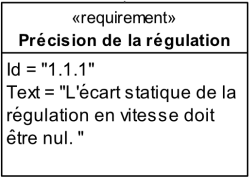
\includegraphics[width=.5\linewidth]{fig_02_bis}

\end{center}

\begin{center}
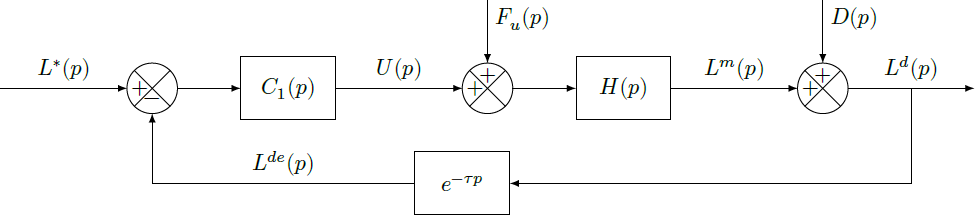
\includegraphics[width=.8\linewidth]{fig_03}

\textit{Figure 1 -- Hélicoptère.}
\end{center}


\begin{center}
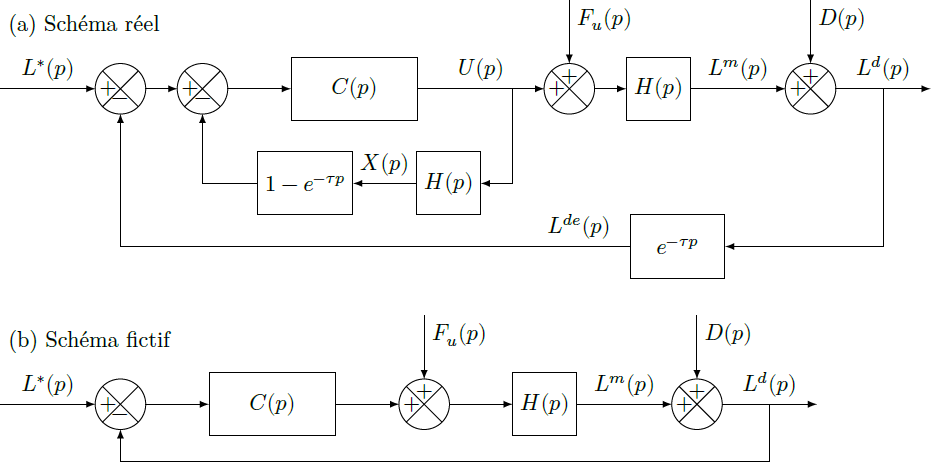
\includegraphics[width=.8\linewidth]{fig_04}

\textit{Figure 2 -- Structure du banc d'essai.}
\end{center}
\fi

\section*{Le moteur à courant continu}
\ifprof
\else
Le banc d'essai est équipé d'un dispositif permettant de générer un couple résistant sur le rotor de sortie de la BTP. Cela permet de simuler les actions aérodynamiques sur les pales. Il faut donc évaluer l'impact de ce couple sur la vitesse du moteur. 
La modélisation adoptée pour le moteur à courant continu est celle de la figure 3.
 
\begin{center}
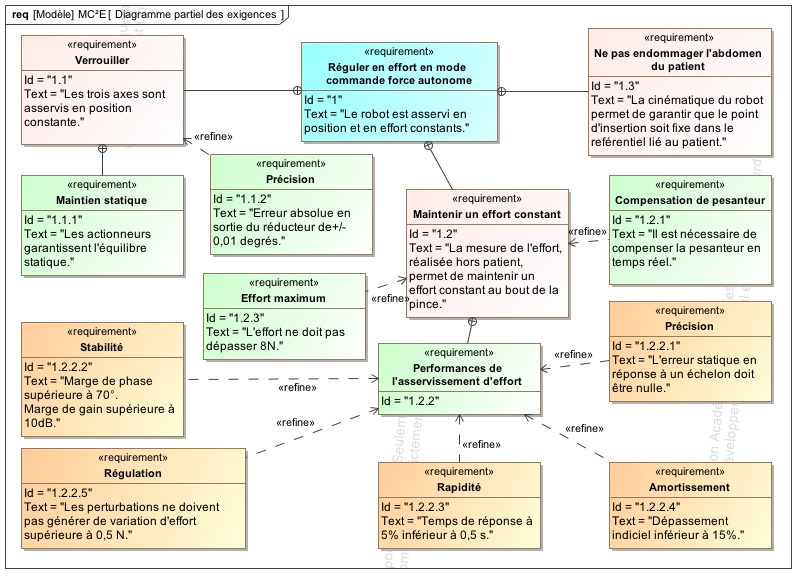
\includegraphics[width=.8\linewidth]{fig_05}

\textit{Figure 3 -- Schéma équivalent du moteur à courant continu.}
\end{center}



On note :
\begin{itemize}
	\item $u(t)$ : la tension appliquée aux bornes de l'induit ;
	\item $i(t)$ : le courant absorbé par l'induit ;
	\item $e(t)$ : la force contre-électromotrice ;
	\item $R$ : la résistance de l'induit ;
	\item $L$ : l'inductance de l'induit ;
	\item $\omega_m (t)$ : la vitesse de rotation de l'arbre moteur ;
	\item $c_m (t)$ : le couple moteur ;
	\item $c_r (t)$ : le couple résistant sur l'arbre moteur dû à la génération d'un couple résistant en sortie de BTP ;
	\item $f$ : le coefficient de frottement, qui génère un couple résistant proportionnel à $\omega_m (t)$ ;
	\item $I_{eq}$ : l'inertie équivalente du banc d'essai ramené à l'arbre moteur ;
	\item $K_c$ : la constante de couple définie telle que
 $c_m (t)=K_c i(t)$	(équation 1);
	\item $K_e$: la constante de force contre-électromotrice définie telle que $e(t)=K_e \omega_m (t)$	(équation 2).
	\end{itemize}
%	
Hypothèses :
\begin{itemize}
\item le comportement de chacun des composants sera considéré comme linéaire, continu et invariant ;
\item les conditions de Heaviside sont considérées comme vérifiées ;
\item on note $p$ la variable de Laplace. La transformée de Laplace d'une fonction temporelle $f(t)$ sera notée $F(p)$ (la transformée de $\omega(t)$ sera notée $\Omega(p)$).
\end{itemize}

\fi

%\question{En justifiant, donner la relation électrique entre $e(t)$, $i(t)$ et $u(t)$.}
%
%On se réfère au schéma cinématique présenté figure 2. On note $I_i$ le moment d'inertie du 
%solide $i$ autour de l'axe de rotation du solide.
%
%\question{Déterminer l'énergie cinétique $E_c (7⁄0)$ de l'ensemble 7 par rapport à 0 en fonction de $\omega(7⁄0)$ et de $I_7$ puis l'énergie cinétique $E_c (6⁄0)$ de l'ensemble 6 par rapport à 0 en fonction de $\omega(7⁄0)$, $Z_7$, $Z_6$ et $I_6$. En déduire l'énergie cinétique $E_c (((6+7))⁄0)$ ainsi que l'inertie équivalente aux solides 6 et 7 (notée $I_{67}$) ramenée sur l'arbre 7.}
%
%Par extension on pourrait déterminer l'inertie équivalente $I_{eq}$ de l'ensemble $E=\{1,2,3,4,5,6,7,BTP\}$ ramenée sur l'arbre moteur 7.
%\question{En utilisant la figure 3 et par la méthode de votre choix, déterminer la relation entre $c_m (t)$, $c_r (t)$, $\omega_m (t)$, $\dfrac{d\omega_m (t)}{dt}$, $I_{eq}$ et $f$.}

%En utilisant le théorème du moment dynamique appliqué à l'arbre en rotation en un point de l'axe et en projection sur l'axe moteur (équation 3):
%$$
%c_m(t)-c_r(t)-f\omega_m(t) = I_{eq} \dfrac{\text{d} \omega_m(t)}{\text{d}t}.
%$$
%
%Enfin, $u(t)=L\dfrac{\text{d}i(t)}{\text{d}t}+Ri(t)+e(t)$ (équation 4).
%
%\question{Traduire dans le domaine de Laplace les équations (1), (2), (3) et (4) . Réaliser alors le schéma bloc associé au moteur à courant continu.}
%
%\question{On fait l'hypothèse que $c_r(t)=0$. Déterminer la fonction de transfert en boucle fermée $\dfrac{\Omega_m(p)}{U(p)}$. Déterminer les constantes caractéristiques d'un système d'ordre 2. }


%\question{Donner la fonction de transfert du moteur et la mettre sous forme canonique en donnant l'expression littérale de chacune des constantes.}
\section*{Modélisation de l'asservissement en vitesse}

\ifprof
\else

Hypothèses :
\begin{itemize}
\item on néglige l'inductance du moteur à courant continu ainsi que l'effet du coefficient de frottement ;
\item on fait l'hypothèse que $K_c=K_e =K$;
\item pour simplifier l'étude, la boucle de courant n'a pas été modélisée.
\end{itemize}
Le schéma-blocs de l'asservissement en vitesse du moteur à courant continu est donné sur la figure 10.
 

\begin{center}
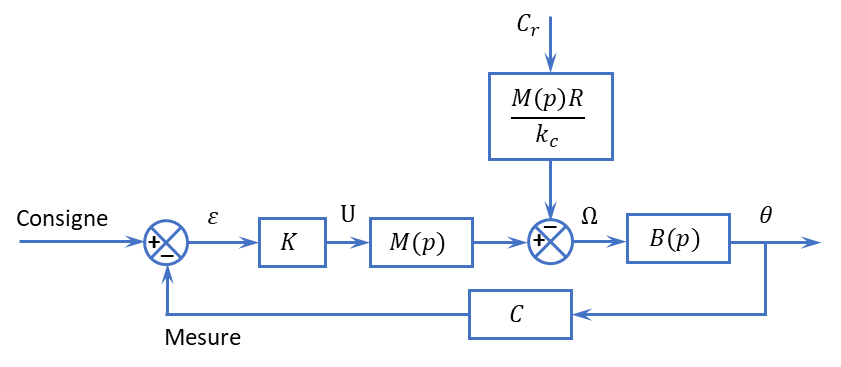
\includegraphics[width=\linewidth]{fig_06}

\textit{Figure 10 -- Régulation en vitesse du banc d'essai.}
\end{center}
\fi

\question{Quelle solution technologique peut-on utiliser pour le capteur situé en boucle de retour ? Comment déterminer la valeur du gain $K_{\text{Adapt}}$ ?}

\ifprof
\begin{corrige}
Il s'agit de réaliser un asservissement en fréquence de rotation. On pourrait utiliser une génératrice tachymétrique. 

Afin d'avoir un asservissement précis ($\varepsilon(p)=0$ lorsque $\Omega_c(p)=\Omega(p)$), on prend $K_{\text{Adapt}}=K_{\text{Capt}}$.
\end{corrige}
\else
\fi


\subsection*{Hypothèse 1 : on considère que $C_r (p)=0$ et $\Omega_c (p)\neq 0$.}
\question{Déterminer la fonction de transfert en boucle fermée $H_m (p)=(\Omega_m (p))/U(p)$ puis la fonction de transfert en boucle fermée $H_1 (p)=(\Omega_m (p))/(\Omega_C (p))$. On considère que $C(p)=K_P$, $K_P$ étant constant. Mettre $H_1 (p)$ sous la forme $K_1/(1+\tau_1 p)$ où on explicitera les valeurs de $K_1$ et $\tau_1$.}

\ifprof
\begin{corrige}
~\\

$H_m (p)=\dfrac{\Omega_m (p)}{U(p)} $
$= \dfrac{\dfrac{K}{RI_{\text{eq}}p}}{1+\dfrac{K^2}{ RI_{\text{eq}}p}}$
$=\dfrac{K}{R I_{\text{eq}} p+K^2  }=\dfrac{1/K}{1+\dfrac{RI_{\text{eq}}}{K^2}p}$


$H_1 (p)=\dfrac{\Omega_m (p)}{\Omega_c (p)} $
$=K_{\text{Adapt}} \dfrac{\dfrac{K}{R I_{\text{eq}} p+K^2 } C(p)}{%
1+\dfrac{K}{R I_{\text{eq}} p+K^2 } C(p) K_{\text{Capt}} }$
$=\dfrac{K_{\text{Adapt}} K C(p)}{R I_{\text{eq}} p+K^2+K C(p) K_{\text{Capt}} }$


$H_1 (p)=\dfrac{K_{\text{Adapt}} K K_P}{R I_{\text{eq}} p+K^2+K K_P K_{\text{Capt}}}$
$=\dfrac{\dfrac{K_{\text{Adapt}} K_P}{K+K_p K_{\text{Capt}}}}{\dfrac{R I_{\text{eq}}}{K^2+K K_P K_{\text{Capt}}} p+1}$
$=\dfrac{K_1}{1+\tau_1 p}$


Soit par identification : $K_1=\dfrac{K_{\text{Adapt}} K_P}{K+K_P K_{\text{Capt}}}$	et	$\tau_1=\dfrac{R I_{\text{eq}}}{K^2+K K_P K_{\text{Capt}}}$.




\end{corrige}
\else

\fi






\subsection*{Hypothèse 2 : on considère que $\Omega_C (p)=0$ et que $C_r (p)\neq0$.}
\question{Retracer sur la copie le schéma bloc en tenant compte de ces hypothèses.}
\ifprof
\begin{corrige}
~\\

\begin{center}
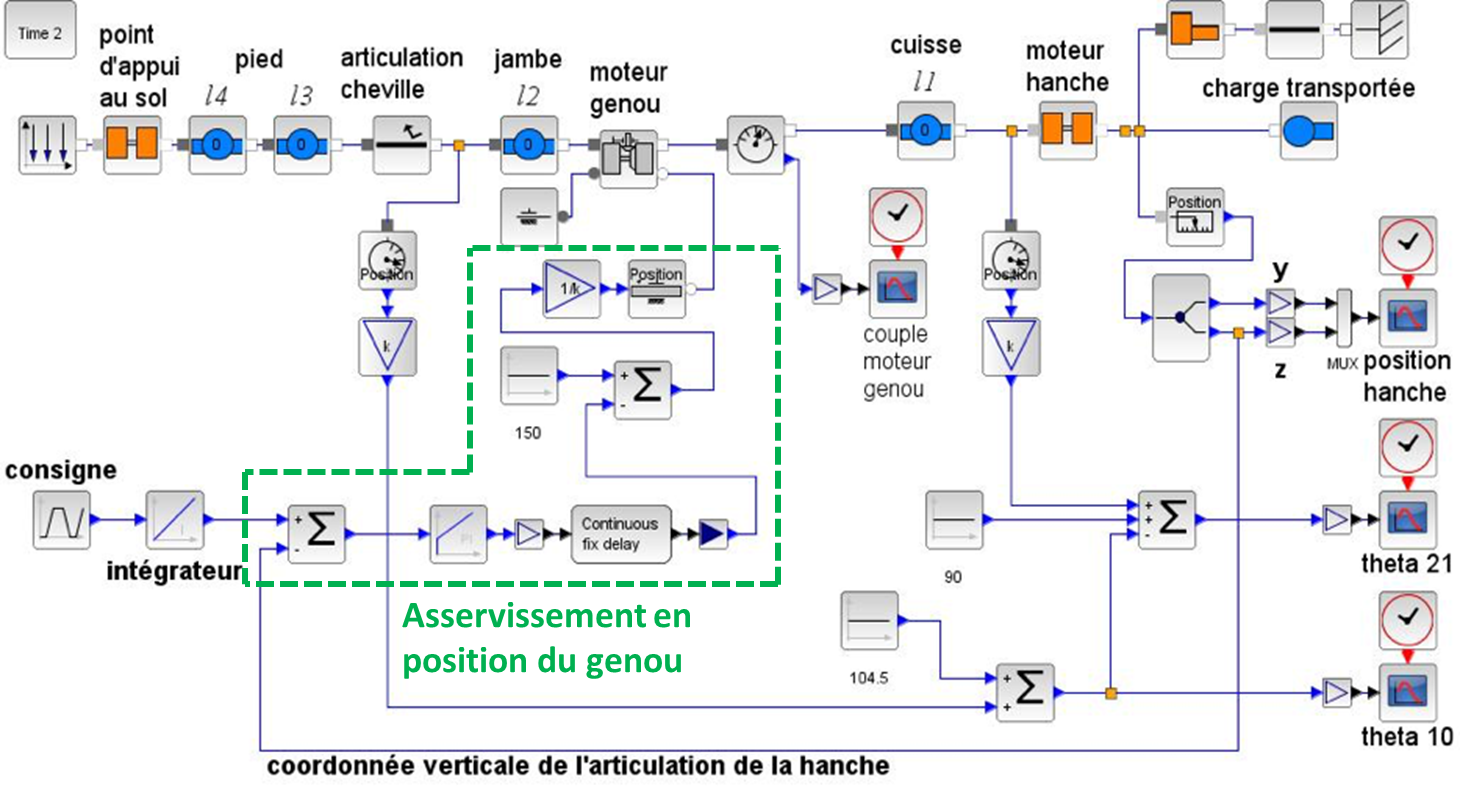
\includegraphics[width=.5\linewidth]{cor_01}
\end{center}
\end{corrige}
\else
\fi


\question{Déterminer la fonction de transfert en boucle fermée $H_2 (p)=(\Omega_m (p))/(C_r (p))$. On considère que $C(p)=K_P$, $K_P$ étant constante. Mettre $H_2 (p)$ sous la forme $-K_2/(1+\tau_2 p)$ où on explicitera les valeurs de $K_2$ et $\tau_2$.}
\ifprof
\begin{corrige}
~\\

\begin{center}
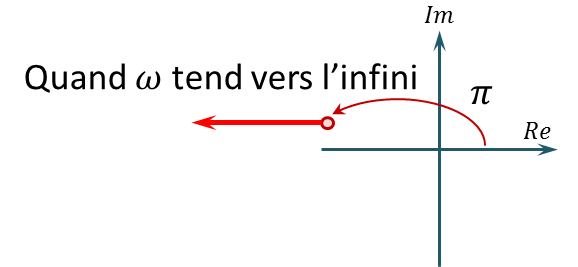
\includegraphics[width=.5\linewidth]{cor_02}
\end{center}
\begin{center}
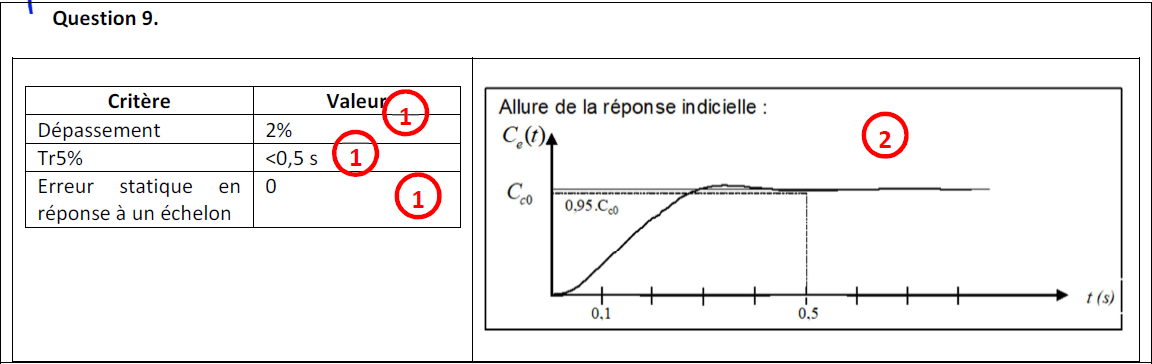
\includegraphics[width=.5\linewidth]{cor_03}
\end{center}
On a donc :	
$H_2 (p)=\dfrac{\Omega_m (p)}{C_r (p)}$
$=-\dfrac{1}{\dfrac{K}{R} \left(K+K_P K_{\text{Capt}} \right)+I_{\text{eq}} p}$
$=-\dfrac{\dfrac{R}{K \left(K+K_P  K_{\text{Capt}} \right) }}{1+\dfrac{R I_{\text{eq}}}{K \left(K+K_P K_{\text{Capt}} \right) } p}$
$=-\dfrac{K_2}{1+\tau_2 p}$
Soit par identification : $K_2=\dfrac{R}{K \left(K+K_P  K_{\text{Capt}} \right) }$	et	$\tau_2=\tau_1=\dfrac{R I_{\text{eq}}}{K (K+K_P K_{\text{Capt}} ) }$.





\end{corrige}
\else
\fi


\subsection*{Hypothèse 3 : on considère maintenant que  $\Omega_C (p)\neq 0$ et que $C_r (p)\neq 0$.}
\question{En utilisant le théorème de superposition, exprimer $\Omega_m (p)$ en fonction de $H_1 (p)$, $H_2 (p)$, $\Omega_c (p)$ et $C_r (p)$.}
\ifprof
\begin{corrige}

Par superposition on a : $\Omega_m (p)=H_1 (p) \Omega_c (p)+H_2 (p) C_r (p)$.
\end{corrige}
\else
\fi


À une fréquence de rotation de $\SI{350}{min^{-1}}$ en sortie de BTP correspond une consigne de fréquence de rotation du moteur de $\SI{1 928}{min^{-1}}$ soit environ $\SI{202}{rad/s}$. Le couple résistant ramené à l'arbre moteur est évalué à $\SI{990}{Nm}$. On soumet donc le système à un échelon de consigne d'amplitude $\SI{202}{rad/s}$ et à un couple résistant de $\SI{990}{Nm}$.

\question{Après avoir exprimé la consigne  $\Omega_c (p)$ puis le couple résistant $C_r (p)$, calculer sous forme littérale l'écart statique du système. Conclure vis-à-vis du cahier des charges.}
\ifprof
\begin{corrige}

On a, pour des échelons de consignes :
$\Omega_c (p)=\dfrac{\Omega_{c0}}{p}$	avec $\Omega_{c0}=\SI{202}{rad/s}$	et	$C_r (p)=\dfrac{C_{r0}}{p}$	avec $C_{r0}=\SI{990}{N m}$.

L’écart statique $\varepsilon_S$  s’écrit en sortie du comparateur :

$\varepsilon_S= \lim\limits_{t\to \infty} \varepsilon(t)$  
$=\lim\limits_{p\to 0} p \varepsilon(p)$
$=\lim\limits_{p\to0} p (K_{\text{Adapt}}\Omega_c (p)-K_{\text{Capt}} \Omega_m (p))$
$=\lim\limits_{p\to 0}  \left(p (K_{\text{Adapt}} \Omega_c (p)-K_{\text{Capt}} H_1 (p) \Omega_c (p)-K_{\text{Capt}} H_2 (p) C_r (p))\right)$

$\varepsilon_S=\lim_{p\to 0}  p \left(K_{\text{Adapt}} \dfrac{\Omega_{c0}}{p}-K_{\text{Capt}} K_1 \dfrac{\Omega_{c0}}{p}+K_{\text{Capt}} K_2 \dfrac{C_{r0}}{p}\right)$

$\varepsilon_S=\left(K_{\text{Adapt}}-K_{\text{Capt}} K_1 \right)\Omega_{c0}+ K_{\text{Capt}} K_2C_{r0}$

L’écart statique ne pourra pas être nul (exigence 1.1.1 du cahier des charges non vérifiée).


\end{corrige}
\else
\fi


\question{Quel intérêt peut présenter l'utilisation d'un correcteur intégral de gain $K_I$ de la forme $C(p)=K_I/p$ ?}
\ifprof
\begin{corrige}
En choisissant $K_{\text{Adapt}}=K_{\text{Capt}}$, l’écart statique pourra être réduit à condition d’avoir un gain $K_P$ important $K_1\to 1$ et $K_2\to 0$, mais pas trop pour ne pas rendre le système instable.
Avec un correcteur intégral, le système devient de classe 1 et l’écart statique est annulé.
\end{corrige}
\else
\fi


\question{En conclusion, en utilisant le correcteur précédent, l'asservissement proposé permet-il de tenir la consigne de vitesse lorsqu'un couple résistant est appliqué à l'arbre de sortie de la BTP ? L'exigence 1.1.1 est-elle vérifiée ?}


\ifprof
\begin{corrige}


En reprenant le raisonnement de la question **, et en remplaçant $C(p)$ par $K_I/p$ dans les expressions de $H_1 (p)$ et $H_2 (p)$ :
$\lim\limits_{p\to 0}  H_1 (p)=\lim\limits_{p\to 0}  K_{\text{Adapt}} \dfrac{\dfrac{K}{R I_{\text{eq}} p+K^2}\dfrac{ K_I}{p}}{1+\dfrac{K}{R I_{\text{eq}} p+K^2 } \dfrac{K_I}{p} K_{\text{Capt}} }$
$=\dfrac{K_{\text{Adapt}}}{K_{\text{Capt}}}$.

$\lim\limits_{p\to 0}  H_2 (p)=\lim\limits_{p\to 0}  -\dfrac{1}{\dfrac{K}{R} \left(K+\dfrac{K_I}{p} K_{\text{Capt}} \right)+I_{\text{eq}} p}=0$

$\varepsilon_S=\lim\limits_{p\to 0}  p \left(K_{\text{Adapt}} \Omega_c (p)-K_{\text{Capt}} H_1 (p) \Omega_c (p)-K_{\text{Capt}} H_2 (p) C_r (p)\right) $

$\varepsilon_S=\lim\limits_{p\to 0} K_{\text{Adapt}} \Omega_{c0}-K_{\text{Capt}} K_{\text{Adapt}}/K_{\text{Capt}}  \Omega_{c0}-K_{\text{Capt}} 0 C_r0 =0$

Dans ce cas, l’application d’un couple perturbateur n’a donc pas d’influence sur l’écart statique. La fréquence de rotation du rotor peut être temporairement impactée, mais au bout d’un laps de temps, l’écart statique tend vers 0. L’exigence 1.1.1 est donc vérifiée.

\end{corrige}
\else
\fi


%\begin{rem}
%On verra ultérieurement qu'un correcteur intégral pur ne permet pas forcément de garantir la stabilité d'un système.
%\end{rem}
%\section*{Partie supplémentaire}
%\question{Tracer le diagramme de Bode de $C(p)\cdot F(p)$ avec $F(p)=118/(1+0,5 p)$ du système lorsque : 
%\begin{itemize}
%\item $C(p)=1$;
%\item $C(p)=20$ ;
%\item $C(p)=30/p$.
%\end{itemize}}

\ifprof
\else
\end{multicols}
\fi